\documentclass[11pt,fullpage]{article}

\usepackage{makeidx,fancyvrb,graphicx}


\newcommand{\alfa}{{\sc Alpha}}
\newcommand{\ammalpha}{{\sc MmAlpha}}
\newcommand{\mmalpha}{{\sc MmAlpha}}
\newcommand{\err}{\top}
\newcommand{\indef}{\bot}
\newcommand{\mma}{{\sc Mathematica}}
\newcommand{\syn}{\texttt{syn}}
\newcommand{\vhdl}{{\sc vhdl}}
\makeindex

\title{The Synthesis Program of \ammalpha{}\\
Version of \today{}}
\author{Patrice Quinton}
\date{Version of July 2008\footnote{There have been modifications since this note was written.}}

\begin{document}
%\bibliographystyle{plain}

\maketitle
%\tableofcontents
%\newpage
\begin{abstract}
This documentation presents the \texttt{syn} command of \ammalpha{}. This command,
which stands for {\em synthesize}, allows an \alfa{} program to be translated into \vhdl{},
whenever possible, by running in a systematic way the commands necessary to transform
the program into \vhdl{}. 
\end{abstract}

\section{Introduction}
\label{Introduction}
The \syn{} command allows a \vhdl{} program to be synthesized directly from
an \alfa{} file. In this document, we explain how this command can be used and
how it is implemented.
To better follow this documentation, you may lauch \mmalpha{} and type 
the command: \texttt{start[]}. A notebook will open, and in this notebook, go in the section
{\em New: synthesis notebooks} where you will find the examples presented
here. 

\section{Basic usage}
\begin{verbatim}
syn[ "file.alpha" ]
\end{verbatim}
in its simplest form. 

However, there are several options that allow the basic method to be changed, if
needed. 

All functions are called with a special parameter \texttt{mute}: by default, they
are silent. 

During the execution of one of the transformation steps, if an error message is triggered, then
\syn{} aborts. It then writes the \alfa{} program in the state that it had when the error 
occured. 

A directory is created where various files produced during the 
synthesis are stored. A trace file, named
\texttt{trace.txt}, contains the list of \mmalpha{} commands that have been executed
until something wrong happened.

Finally, if everything goes well, a report file is written in this directory. 

Example:
\begin{verbatim}
syn["fir.alpha"]
\end{verbatim}
synthesizes the program contained in file \texttt{file.alpha}, 
and shown in Appendix~\ref{firprogram}.

This basic command stops just before generating \vhdl{}, as the values of the 
\texttt{K} and \texttt{M} parameters are not set. To obtain \vhdl{}, run 
\begin{verbatim}
syn["fir.alpha", parameterRules -> {"N" -> 20, "M" -> 100}]
\end{verbatim}

The synthesis is almost silent, and takes a few seconds. If it succeeds, a 
congratulation message is issued\footnote{You'll understand why when you
start synthesizing you own program!}.

You get more information by adding the \texttt{verbose} option:
\begin{verbatim}
syn["fir.alpha", parameterRules -> {"N" -> 20, "M" -> 100}, 
  verbose->True]
\end{verbatim}

The \texttt{syn} program has a few options that can be displayed by
evaluating \texttt{Options[ syn ]}.

\subsection{The \texttt{SYN} directory}
The execution creates a directory named \texttt{"firSYN"} which contains: 
\begin{itemize}
\item \texttt{fir.report}: a file giving an analysis of the program after the 
\texttt{Alpha0} code generation (corresponding to the file 
\texttt{firAlpha0.alpha"}. 
\item \texttt{fir.scd}: the value of the schedule that was produced and used.
\item \texttt{firAlpha0.alpha}: the program, after \texttt{Alpha0} generation.
\item \texttt{firAlphard.alpha}: the program, after \texttt{Alphard} generation.
\item \texttt{firParametersFixed.alpha}: the program, after parameters are fixed. This is
the last transformation step before \vhdl{}�generation.
\item \texttt{firPiped.alpha}: the program, after piping variables.
\item \texttt{firScheduled.alpha}: the program, after scheduling and placement.
\item \texttt{trace.txt}: the list of \mmalpha{}�commands executed.
\item \texttt{VHDL}: a directory that contains the \vhdl{} programs.
\end{itemize}

If the directory contains a file including \texttt{Wrong} in its name, then one of
the steps went wrong (or maybe, this was produced during a previous execution 
of \texttt{syn}, as the directory is not cleaned.) 

\section{The \texttt{VHDL} Directory}
The \texttt{VHDL} directory contains the following files, if the synthesis was
successful: 
\begin{itemize}
\item \texttt{ControlfirModule.component}: the component description of the 
controller part.
\item \texttt{ControlfirModule.vhd}: the \vhdl{} description of the controller part.
\item \texttt{cellfirModule1.component}: the component description of the first cell.
\item \texttt{cellfirModule1.vhd}: the \vhdl{} description of the first cell.
\item \texttt{cellfirModule2.component}: the component description of the second cell.
\item \texttt{cellfirModule2.vhd}: the \vhdl{} description of the first cell.
\item \texttt{cellfirModule4.component}: the component description of cell number 4.
\item \texttt{cellfirModule4.vhd}: the \vhdl{} description of cell number 4.
\item \texttt{definition.vhd}: a useless file.
\item \texttt{fir.component}: the component description of the fir.
\item \texttt{fir.vhd}: the \vhdl{} description of the fir filter.
\item \texttt{firModule.component}: the component description of the 
module part.
\item \texttt{firModule.vhd}: the \vhdl{} description of the module part.
\end{itemize}
The generation of \vhdl{} follows the structure shown in Fig.~\ref{firvhdl}. The main 
file, \texttt{fir.vhd}, may not be usable for reasons that are difficult to explain here...
But \vhdl{} file called \texttt{firModule.vhd} should be synthesizable. It calls a 
controller and instanciates three types of basic cells. 
\begin{figure}[ht]
\centerline{
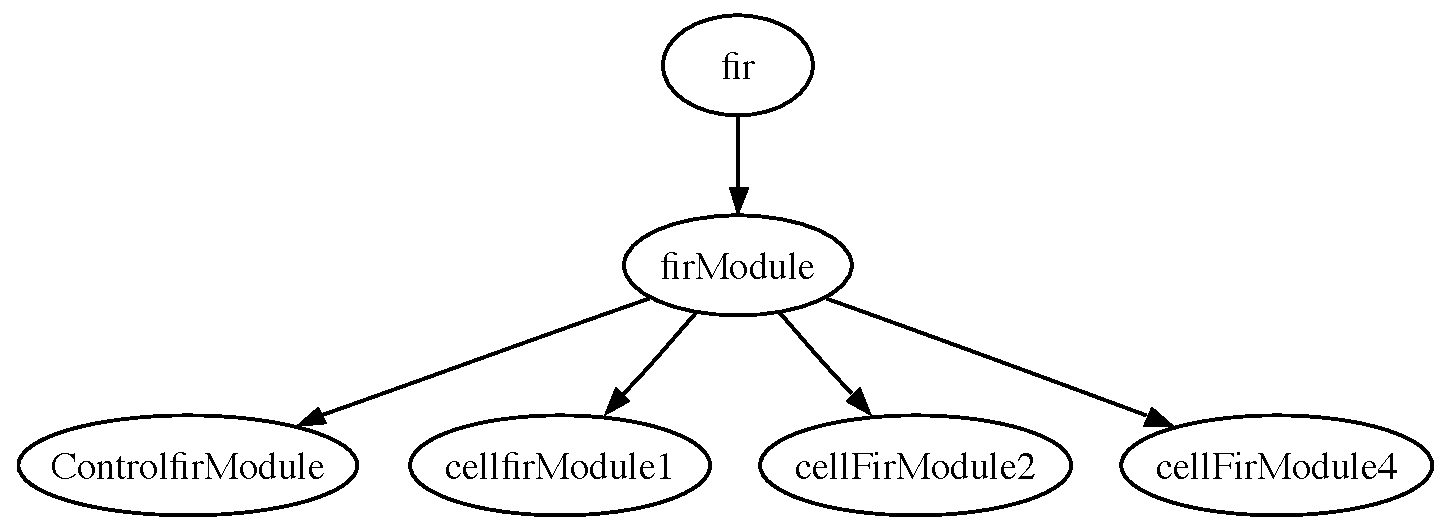
\includegraphics[width=\textwidth]{firvhdl.pdf}
}
\caption{Structure of \vhdl{} generated for the FIR filter\label{firvhdl}}
\end{figure}

\section{What \syn{} does}
\begin{enumerate}
\item Loads the specified file. If this step is successful, the {\em synthesis directory} is created. Its
name is \texttt{xxxSyn} where \texttt{xxx} is the name of the local directory.
\item Inline program, if needed. In other words, if the loaded program contains several
systems, then the last one that was loaded is inlined. If this step is successful, then
only this last system is kept in the library, and it is saved under the name \texttt{yyyInlined.alpha}
in the synthesis directory, where \texttt{yyy} is the name of this system.
\item Checks the program, by doing a static analysis.
\item Schedule the program. Without options, \texttt{schedule[]} is applied. Options can 
be provided (see Section~\ref{options}) to either call \texttt{scd[]}�and give 
hints to the scheduler. Found schedule is saved in the synthesis directory and if no 
schedule is found, the file is saved under the name \texttt{yyyWrongScheduled.alpha}.
\item Applies the schedule. Result is saved in file \texttt{yyyScheduled.alpha}.
\item Pipes variables using \texttt{pipeVars} command. 
Result is saved in file \texttt{yyyPiped.alpha} (or \texttt{yyyWrongPiped.alpha} if an
error occured).
\item Generates 
\end{enumerate}

\section{Options}
\label{options}
\begin{description}
\item[\texttt{optionsOfScheduler}:] contains options that are passed to the scheduler
\item[\texttt{debug}:] debug option
\item[\texttt{verbose}:] 
\item[\texttt{schedMethod}:] allows the scheduler type to be specified. Values are 
\texttt{farkas} (by default) or otherwise (any other value), the vertex method.
\item[\texttt{parameterRules}:] specifies an association list of parameter values.
\end{description}
 
\section{Report}
\label{report}
\begin{enumerate}
\item Writes \texttt{Equation}
\item Gives the declaration of the lhs
\item Prints out the equation
\item Prints out the type of the lhs
\item Signals if equation is an output equation (the lhs is an output variable), or a local
equation (the lhs is local)
\item Signals if we have an input equation, i.e., an equation of the form \texttt{lhs = input}\footnote{This should be extended to the case where there is an domain, and possibly an dependency.}.
\item Prints out the indexes.
\item Signals if equation is scheduled. It could be a scalar, a variable with one dimension of
time, possibly with several dimensions of space.

\end{enumerate}

\appendix
\newpage
\VerbatimInput{fir.alpha}
%\newpage
\section{\vhdl{} Model Generated for the FIR Module}
This is the file \texttt{firModule.vhd}. 
\VerbatimInput{firModule.vhd}
\section{\vhdl{} Model Generated for the FIR cell 2}
This is the file \texttt{cellfirModule2.vhd}. 
\VerbatimInput{cellfirModule2.vhd}

%\bibliographystyle{alpha}
%\bibliography{biblio}
\printindex

\end{document}
